\documentclass[10pt]{article}
% for editing use
%\usepackage{lineno}
%\linenumbers
%\usepackage{endfloat}

% minimal packages here
\usepackage{listings}
\usepackage{booktabs}
\usepackage[noadjust]{cite}
\bibliographystyle{IEEEtran}
\usepackage[plain]{fancyref}
\renewcommand{\freffigname}{Fig.}
\renewcommand{\Freffigname}{Fig.} 
\renewcommand{\freftabname}{Table}
\renewcommand{\Freftabname}{Table}
\frefformat{plain}{\fancyrefeqlabelprefix}{(#1)} 
\Frefformat{plain}{\fancyrefeqlabelprefix}{(#1)} 
\usepackage{siunitx}
\usepackage{graphicx}
\usepackage{hyperref}
\hypersetup{%
	colorlinks=true,
	linkcolor=violet,
	urlcolor=blue,
	citecolor=blue,
	pdfauthor={Corwin Stites},
	pdftitle={Unmanned underwater vehicle mobile mesh networks: applications for hydrographic surveying},
	pdfsubject={weapons, robotics, and control engineering},
	pdfkeywords={UUV, mesh networks, hydrographic survey}}

% for editing use
\usepackage{color}
\definecolor{mygreen}{RGB}{28,172,0}
\definecolor{mylilac}{RGB}{170,55,241}
\usepackage[colorinlistoftodos]{todonotes}

% Fall Smester Bowman Research Report
\title{Unmanned Underwater Vehicle Mobile Mesh Networks: Applications for Hydrographic Surveying}
\author{Corwin W. Stites\thanks{Author is with the Department of Weapons, Robotics, and Control Engineering at the United States Naval Academy. Address for correspondence: \emph{m216468@usna.edu}}}
\date{December 1, 2020}

\begin{document}

\maketitle

\begin{abstract}
	Underwater surveying is a costly and time consuming endeavor. My project is investigating how a mobile mesh network could be applied to make hydrographic surveys more efficient and accurate. Such a network would consist of a group of sonar equipped Unmanned Underwater Vehicles (UUVs) connected via a mesh network actuated through an acoustic modem. The project focus is on the spatial arrangement of the nodes as well as how nodes of the mesh network would communicate for best effect to accomplish fast hydrographic surveying of a predetermined area or fast location of an underwater target of interest.  
\end{abstract}

{\scriptsize\textbf{Keywords: } UUV, Mesh Networks, Hydrographic Survey}

\section{Motivation}
Underwater surveying is a critically important yet resource intensive endeavour. Large areas of ocean must have bathymetry data regularly updated in order to allow for safe ship navigation. Furthermore, finding a submerged target such as a wreckage or explosive device  requires large areas of ocean to be surveyed. Unmanned Underwater Vehicles have proven success in greatly streamlining the hydrographic surveying process by allowing for collaborative fleet surveying. Creating a mobile network of UUVs provides opportunities for further autonomization of hydrographic surveying.  A mesh network made up of UUVs acting as individual nodes would allow for collaborative position and velocity tracking within the network thus removing the need for constant shipboard control. When designing such a network, redundancy in the network will be a critical aspect of the design. In other words, the network must be able to route around missing nodes in the event that a UUV is damaged or goes offline.


\section{Research Introduction}
The aim of this research was to investigate the redundancy of different UUV mesh networks built for the purpose of conducting hydrographic surveying. The research determined how the spatial arrangement of nodes in a network and the connection architecture of the network would affect the ability of a network to function in the event of multiple offline nodes. \par 
The metrics used to measure this in the project was the successful connection rate between two nodes in a damaged network and the average path length of successful connections. This data was taken from 100 random pairs of nodes in a randomly damaged network. The ratio of successful connections to total connection attempts was measured and deemed the "Survivability Rate." Out of the successful connections the sum of the paths' lengths that formed the connection was measured. This was then averaged for all successful connections and deemed the "Surviving Path Length." This value could be used to determine latency time since it could be used to determine the travel time of an acoustic signal based on an approximate value of the speed of sound in saltwater. \par 
Three types of network spatial arrangements were investigated each with a different connection architecture protocol. This portion of the project was important for laying the groundwork of developing methods for building and testing networks in a coding environment in order to begin further exploring more advanced topics like healing algorithms, network throughput, and data rates next semester. 


\section{Methods}
The method of testing was software simulation. The code was written in Python utilizing the NetworkX library to build and simulate the networks. A few key control variables were set during the tests. All networks were arranged in a 40 meter squared operating area. All networks were also built with thirty nodes and five nodes were removed from each network to simulate a damaged network. \par

Before the simulation could be run, the networks and and their connection protocols had to be built. The first network was a completely randomly distributed network that utilized an opportunistic routing algorithm to form its connections. The opportunistic routing algorithm functioned by finding the best opportunity for each connection while ensuring that all nodes were connected to the network. This entailed connecting every node to the closest node that it did not have an existing connection with.The intent of this network was to be a basis of comparison for other networks utilizing more advanced and formulaic architectures. The next network was a circular network arranged around a master node. This entailed the master node being surrounded by two concentric rings of worker nodes. The master node was connected to all members of the inner ring while members of the inner ring only connected to members of the outer ring that was within a particular distance threshold. The final network was a square grid layout of evenly spaced nodes. Connections were only formed with nodes aligned vertically above or horizontally to the side of a particular node. \par

\begin{figure}
\begin{center}
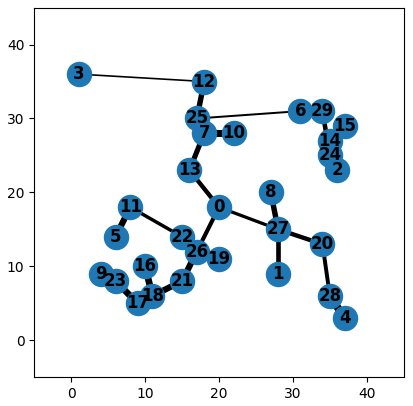
\includegraphics[width=0.33\columnwidth]{figures/RandomLayout.png}
\end{center}
\caption{A NetworkX generated plot showing a randomly distributed network of 30 nodes connected with an opportunistic protocol. Note: Weight of the line indicates the connection latency or distance between nodes.}
\end{figure}

\begin{figure}
\begin{center}
\includegraphics[width=0.33\columnwidth]{figures/MasterLayout.png}
\end{center}
\caption{A plot showing a circular network utilizing a master node at the center.}
\end{figure}

\begin{figure}
\begin{center}
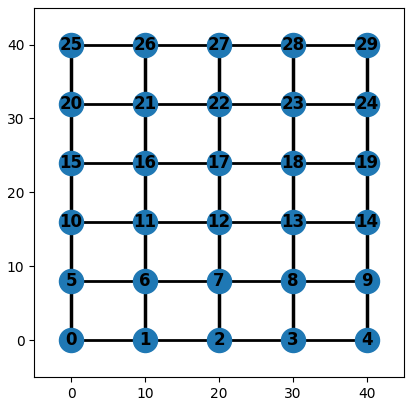
\includegraphics[width=0.33\columnwidth]{figures/GridLayout.png}
\end{center}
\caption{A plot showing a grid network with only adjacent vertical and horizontal connections.}
\end{figure}

Next an array of randomly damaged networks had to be created to be run through the function that would determine the network architectures. A function was created that took and undamaged network as an argument and randomly removed five of its nodes and all connections to or from those nodes. This produced the damaged networks that would be used in the simulation.\par

\begin{figure}
\begin{center}
\includegraphics[width=0.33\columnwidth]{figures/DamagedRandomLayout.png}
\end{center}
\caption{A plot showing a damaged random network.}
\end{figure}

\begin{figure}
\begin{center}
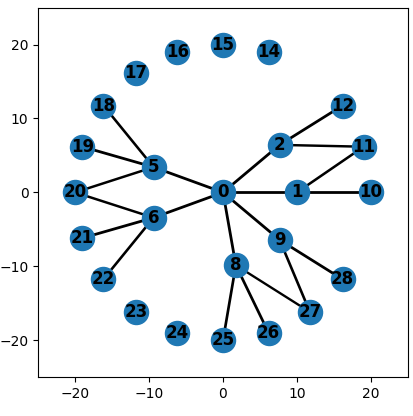
\includegraphics[width=0.33\columnwidth]{figures/DamagedMasterLayout.png}
\end{center}
\caption{A plot showing a damaged master network.}
\end{figure}

\begin{figure}
\begin{center}
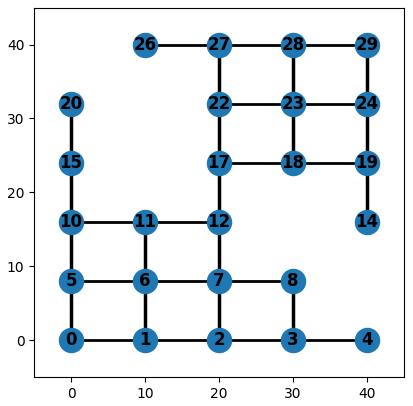
\includegraphics[width=0.33\columnwidth]{figures/DamagedGridLayout.png}
\end{center}
\caption{A plot showing a damaged grid network.}
\end{figure}

To test the damaged networks, the simulation ran 1000 iterations of collecting the average survivability rate and the surviving path length from 100 randomly damaged networks. Using an average velocity of sound in saltwater of 1510 meters per second the average travel latency of the acoustic signal was calculated from the average path length.

\section{Pseudo Code}
The following pseudo code provides a basic overview of how the code tests the survivability of various mesh network layouts. 
\lstset{basicstyle=\footnotesize}
\begin{lstlisting}

Define Create_Network_Function()
	return desired_network_layout
Define Delete_Nodes_Function(Network)
	i = 0
	while 1=<5
		delete random node in Network 
		i=i+1
	return damaged_network
Define Find_Survivability/Latency_Function(Damaged_Network)
	i = 0
	while 1=<100
		Pick two random nodes in Damaged_Network
		Find if path exists or not between them
		If path exists find the length
		i = i+1
	Survivability = Find ratio of successful connections to... 
	total connection attempts
	Path_Length = Find average surviving path length
	return [Survivability, Path_Length]

i = 0
while 1=<1000
	Network = Create_Network_Function()
	Damaged_Network = Delete_Nodes_Function(Network)
	[Survivability[i], Path_Length[i]]...
	= Find_Survivability/Latency_Function(Damaged_Network)
	i = i+1
Final_Values = Average([Survivability, Path_Length])
\end{lstlisting}

\section{Results}
The results of the simulation showed that the random network performed least well over both aspects of the simulation. This result was expected as the random network was intended mostly as a basis for comparison. The master network demonstrated the lowest surviving connection path length, and consequently, the lowest acoustic signal travel latency.  This is due to the circular arrangement allowing pseudo-diagonal connections across the testing area compared to the grid network’s vertical and horizontally aligned connections. In terms of survivability however, the grid network’s repetitive communication architecture proved to have superior redundancy over the master network. This is  due to the fact that the master network is heavily reliant on the master node for its connection architecture as it it is the only path between the inner circle of worker nodes. If the master nod is removed, the network is very vulnerable to connection failure.  

\begin{figure}
\begin{center}
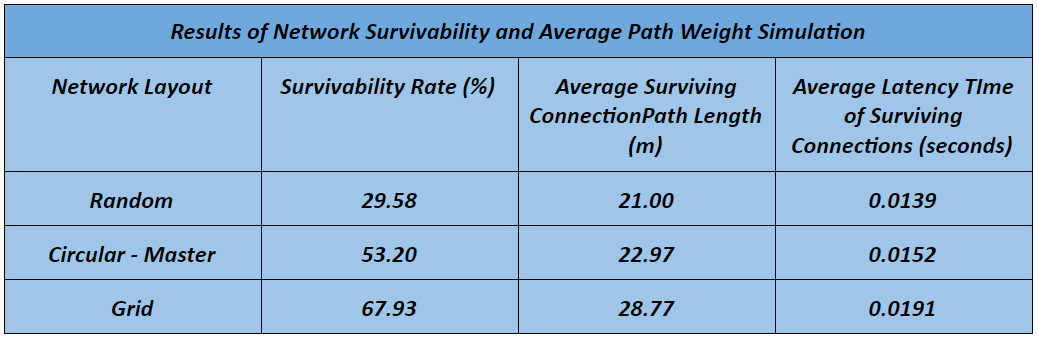
\includegraphics[width=0.6\columnwidth]{tables/ResultsTable.PNG}
\end{center}
\caption{A table showing the simulation results for each network type.}
\end{figure}

\begin{figure}
\begin{center}
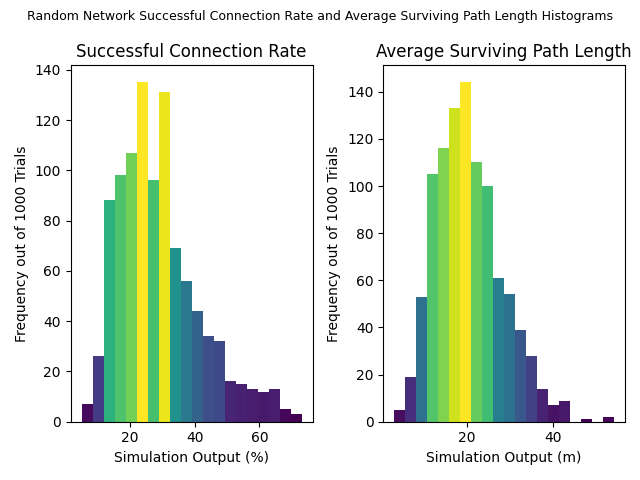
\includegraphics[width=0.6\columnwidth]{figures/RandomHistogram.png}
\end{center}
\caption{A histogram showing the simulation result distribution for the random network.}
\end{figure}

\begin{figure}
\begin{center}
\includegraphics[width=0.6\columnwidth]{figures/MasterHistogram.png}
\end{center}
\caption{A histogram showing the simulation result distribution for the master network.}
\end{figure}

\begin{figure}
\begin{center}
\includegraphics[width=0.6\columnwidth]{figures/GridHistogram.png}
\end{center}
\captionA {A histogram showing the simulation result distribution for grid network.}
\end{figure}

\section{Discussion}
The results of the simulation show that a circularly arranged master node network has advantages in terms of reducing travel latency while a grid network provides an advantage in survivability. A user could choose between these networks based on the perceived threat to the network and/or desired transmission speed within the network. A single network could also be designed to incorporate aspects from both  (including diagonal connections in the grid algorithm for example) in order to combine the strengths of the two networks. While the results of this simulation were not particularly surprising, the process of building the networks and simulations laid the groundwork for deeper research questions that will be explored next semester regarding additional network spatial arrangements as well as more advanced routing protocols and network healing algorithms.

\end{document}


% Copied from poster by DE
%\section*{Introduction}
%Underwater surveying is a costly and time consuming endeavor. Large areas of ocean must have bathymetry data regularly updated in order to allow for safe ship navigation. Furthermore, finding a submerged target such as a wreckage or explosive device  requires large areas of ocean to be surveyed. Unmanned Underwater Vehicles have proven success in greatly streamlining the hydrographic surveying process by allowing for collaborative fleet surveying. Creating a mobile network of UUVs provides opportunities for further autonomization of hydrographic surveying.  A mesh network made up of UUVs acting a sindividual nodes would allow for collaborative position and velocity tracking within the network  thus  removing the need for constant shipboard control. When designing such a network, redundancy in the network will be a critical aspect of the design. In other words, the network must be able to route around missing nodes in the event that a UUV is damaged or goes offline.
%\begin{figure}
%\begin{center}
%image here
%\end{center}
%\caption{An example of fleet UUV network technology. Ocean Infinity Hugin AUVs conducting hydrographic surveying while being controlled by a ship mounted acoustic modem.}
%\end{figure}
%
%\subsection*{Problem statement}
%The aim of this research was to investigate the redundancy of different UUV mesh networks built for the purpose of conducting hydrographic surveying. The research determined how the spatial arrangement of nodes in a network and the connection architecture of the network would affect the ability of a network to function in the event of multiple offline nodes. Three types of network spatial arrangements were investigated each with a different connection architecture protocol. 
%\begin{enumerate}
%\item A network of randomly distributed nodes using an opportunistic connection algorithm (connection formed between closest nodes). 
%\item A network made up of a ``master node'' surrounded by two concentric circles of worker nodes connected by a branching algorithm.
%\item A grid network connected by a grid algorithm. 
%\end{enumerate}
%
%\section*{Methods and materials}
%The method of testing was software simulation. The code was written in Python utilizing the \lstinline{networkx} library to build and simulate the networks. A few key control variables were set during the tests.
%\begin{enumerate}
%\item All networks were arranged in a \SI{40}{\meter\squared} operating area.
%\item All networks were built with 30 nodes.
%\item 5 nodes were removed from each network to simulate a damaged network.
%\end{enumerate}
%The simulation ran 1000 iterations of collecting the average survivability (successful connection rate between two random nodes) and the average surviving connection length from 100 randomly damaged networks. Using an average speed of sound in saltwater of  $V_{sound} = \SI{1510}{\meter\per\second}$, the average travel latency of the acoustic signal was calculated from the path length.
%
%\begin{figure}
%\begin{center}
%Code block here
%\end{center}
%\caption{Pseudocode providing a basic synopsis of the simulation code}
%\end{figure}
%
%\begin{figure}
%\begin{center}
%image here
%\end{center}
%\caption{NetworkX Plots showing from left to right a randomly distributed network, a circular master node network, and a grid network.}
%\end{figure}
%
%\begin{figure}
%\begin{center}
%image here
%\end{center}
%\caption{NetworkX Plots showing the above networks after having been run through a function to randomly remove five nodes.}
%\end{figure}
%
%\section*{Results}
%\begin{table}
%\caption{Table of simulation outputs. Results of network sensitivity and average path weight simulation.}
%\begin{center}
%  \begin{tabular}{cccc}
%    \toprule
%    network layout & survivability rate (\si{\percent}) & average surviving connection path length (\si{\meter}) & average travel latency time of surviving connections (\si{\second})\\
%    \midrule
%    random & 25.98 & 21.00 & 0.0139\\
%    circular-master & 53.20 & 22.97 & 0.0152 \\
%    grid & 67.93 & 28.77 & 0.0191 \\
%    \bottomrule
%    \end{tabular}
%\end{center}
%\end{table}
%
%\begin{figure}
%\begin{center}
%image here
%\end{center}
%\caption{Histograms showing the frequency of successful connection rates and average surviving path lengths out of 1000 trials for each graph type.}
%\end{figure}
%
%\section{Discussion}
%\begin{block}{Discussion}
%The results of the simulation showed that the random network performed least well over both aspects of the simulation. This result was expected as the random network was intended mostly as a basis for comparison. The master network demonstrated the lowest surviving connection path length, and consequently, the lowest acoustic signal travel latency.  This is due to the circular arrangement allowing pseudo-diagonal connections across the testing area compared to the grid networks vertical and horizontally aligned connections. In terms of survivability however, the grid networks repetitive communication architecture proved to have superior redundancy over the master network. 
%
%The results of the simulation show that a circularly arranged master node network has advantages in terms of reducing travel latency while a grid network provides an advantage in survivability. A user could choose between these networks based on the perceived threat to the network and/or the user’s desired network transmission speed within the network. One network could also be designed to incorporate aspects from the other (including diagonal connections in the grid algorithm for example) in order to combine the strengths of the two networks. While the results of this simulation were not particularly surprising, the process of building the networks and simulations laid the groundwork for deeper research questions that will be explored next semester regarding additional network spatial arrangements as well as more advanced routing protocols and network healing algorithms.
%
%\section*{Acknowledgements}
%
%%\section*{References}
%%\begin{block}{References}
%%\bibliographystyle{IEEEtrans} % or IEEEtrans if you want that kind
%%\scriptsize\bibliography{poster.bib}
%%\end{block}
%
